\documentclass[12pt]{article}
\usepackage{amsmath, amsthm, amsfonts, amssymb}
\usepackage{graphicx} % for images
\usepackage{hyperref}

% Define theorem and lemma environments
\newtheorem{theorem}{Theorem}
\newtheorem{lemma}{Lemma}
\newtheorem{definition}{Definition}

\setlength{\parindent}{0pt}

\begin{document}

\title{[UltraReps] Bayesian-Optimal Multi-Classification with Noisy Input Necessitates General Input Space Representation}

\author{Aman Bhargava}

\date{\today}
\maketitle

\section{Introduction}
\label{sec:intro}
\textit{Notation: lower case variables denote scalars (e.g., $x$), upper case variables denote random variables (e.g., $X$), and boldfaced variables denote vector quantities (e.g., $\mathbf x, \mathbf X$). 
We denote the $d\times d$ identity matrix as $\mathbf I_d$.} \\

Here we analyze the latent representations in optimal Bayesian filter models trained to perform multi-classification on some ground truth input vector $\mathbf x^* \in \mathbb R^d$ based on noisy discrete-time measurement signals $\mathbf X(1), \dots, \mathbf X(t)$ for i.i.d. $\mathbf X(i) = \mathbf x^* + \mathcal N(\mathbf{0, I_d})$. Classification boundaries are denoted $\{(\mathbf c_i, b_i)\}_{i = 0}^M$ where $\mathbf c_i \in \mathbb R^d$ is the normal vector to the hyperplane and $b_i\in \mathbb R$ is the offset from the origin. 
For boundary $i$, the separating plane defined as the affine set $\{\mathbf x | \mathbf c_i^\top \mathbf x = b_i\}$. 
The ground truth classification of a given point $\mathbf x$ is given by decision rule $y(\mathbf x)$: 

\begin{equation}
	\label{def:decision_rule}
	y_i(\mathbf x) = \begin{cases}
		1 & \text{ if } \mathbf c_i^\top \mathbf x > b_i \\ 
		0 & \text{ otherwise } 
	\end{cases}
\end{equation}



\begin{figure}[h! tbp]
	\centering 
	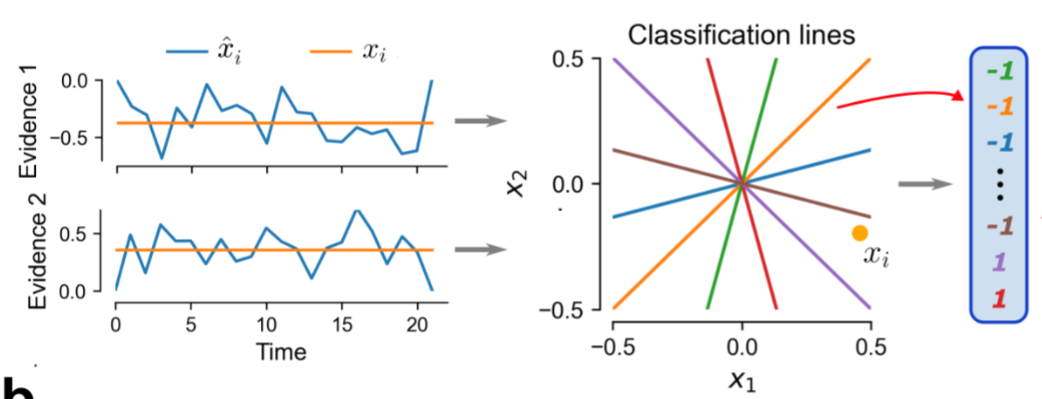
\includegraphics[width=0.9\textwidth]{media/multitask_fig2a.png}
	\caption[Multitasking RNN learns abstract representations]{\textbf{Multitasking RNN learns abstract representations. } Data generating process. The task is to simultaneously report whether the true joint evidence $(x_1,x_2)$ (yellow dot) lies above ($+1$) or below ($-1$) a number of classification lines (here 6).}
	\label{fig:2a}
\end{figure}

A restricted form of the problem is depicted in Figure~\ref{fig:2a}. Note that we are interested in the general case where the hyperplanes do not necessarily pass through the origin. 




\section{Bayesian Filtering Framework}
\label{sec:bayes_framework}

We are interested in the properties of optimal Bayesian filter models that sequentially process inputs $\mathbf X(t)$ to estimate each classification $y_i(\mathbf x^*), i\in [M]$. 
Bayesian filters are a class of statistical models and algorithm that update a latent state based on noisy and uncertain observation signals. 
Rooted in principles of Bayesian inference, these filters combine aggregated ``knowledge'', represented by a latent state $\mathbf Z(t)$, with incoming observations $\mathbf X(t)$ to continually update the latent state to facilitate some prediction of some output $\mathbf Y(t) = f(\mathbf Z(t))$. 


\begin{definition}[Bayesian Filter Operation]
	\label{def:bayesian_filter}
	A discrete-time Bayesian filter updates latent variable $\mathbf z(t)$
	based on incoming data $\mathbf x(t)$ by applying Bayes' theorem: 
	\begin{align}
		\label{eqn:bayes_filter}
		P \big(\mathbf z(t) | \mathbf  x(t), \mathbf z(t-1)\big) &= \frac{
			P\big(\mathbf x(t) | \mathbf z(t), \mathbf z(t-1)\big) 
			P\big(\mathbf z(t) | \mathbf z(t-1)\big)
		}{
			P\big(\mathbf x(t) | \mathbf z(t-1)\big)
		} \\
		&\propto P\big(\mathbf x(t) | \mathbf z(t) \big) 
			P\big(\mathbf z(t) | \mathbf z(t-1)\big)
	\end{align}
	Bayesian filters are commonly equipped with a ``decoder'' or ``readout
	map'' $f$ which maps latent $\mathbf Z(t)$ to readout estimation
	$\hat{\mathbf Y}(t) = f(\mathbf Z(t))$.
\end{definition}


The readout $\hat{\mathbf Y}(t)$ is a vector of Bernoulli random variables with index $i$ corresponds to the estimate of classification $(\mathbf c_i, b_i)$. 










\section{Main Result}

In this section we show that an optimal Bayesian filter performing multi-classification as described in Section~\ref{sec:intro} must store a representation of $x^*$ in the latent variable $\mathbf Z(t)$. 
More specifically, we show that the maximum likelihood estimate of $x^*$ based on $\mathbf X(1), \dots, \mathbf X(t)$ is recoverable from $\mathbf Z(t)$.



\subsection{Single Decision Boundary}
\label{sec:single_boundary}

First, we will consider the Bayesian filtering of a single classification output $y(x^*)$ from noisy inputs $X(1), \dots, X(n)$ with decision boundary parameters $(\mathbf c, b)$. 
We begin by scaling our coordinates such that the Gaussian noise has unit variance:
\begin{equation}
	\mathbf X(t) = \mathbf x^* + \mathcal N(\mathbf{0, I_d})
\end{equation}
The problem is further simplified by setting $b = 0$. 
We are interested in $P(\hat Y(t) | \mathbf X(1), \dots, \mathbf X(t))$ where $\hat Y(t)$ is a Bernoulli random variable representing the probability that $y(\mathbf x^*) = 1$ given evidence $\mathbf X(1), \dots, \mathbf X(t)$. 

Since $y(\mathbf x^*)$ is a deterministic function of non-random variable $x^*$, we will first derive the probability distribution over $\mathbf x^*$ (denoted $\hat{\mathbf X}$) to determine $y(\hat{\mathbf X})$. 

\begin{lemma}
	\label{lemma:x_star_estimate}
	For $\mathbf X(t) = \mathbf x^* + \mathcal N(\mathbf{0, I_d})$ and no prior on $x^*$, the conditional probability distribution $\hat{\mathbf X} = P(x^* | \mathbf X(t), \dots, \mathbf X(t))$ is given by 
	\begin{equation}
		\hat{\mathbf X} = \mathcal N(\hat \mu, \hat \Sigma)
	\end{equation}

	where $\hat \mu$ is the mean of $\mathbf X(1), \dots, \mathbf X(t)$ and $\hat \Sigma = t^{-1/2} \mathbf I_d$. 

	\begin{proof}
		Since $\mathbf X(1), \dots, \mathbf X(t)$ are i.i.d. from a Gaussian distribution with mean $\mathbf x^*$ and identity covariance, the sample mean is known to be distributed normally centered at the ground truth $\mathbf x^*$. 
		We apply the known standard deviation of the underlying distribution (identity covariance) to arrive at $\hat \Sigma = t^{-1/2} \mathbf I_d$ as the standard deviation on the sample mean (derived from the central limit theorem). 
	\end{proof}
\end{lemma}


We can use estimator $\hat{\mathbf X}$ to construct $\hat{\mathbf Y}$ by expanding $\hat{\mathbf Y} = y(\hat{\mathbf X})$ as 
\begin{equation}
	y(\hat{\mathbf X}) = \begin{cases}
		1 & \text{ if } \mathbf c^\top \hat{\mathbf X} > 0 \\ 
		0 & \text{ otherwise } 
	\end{cases}
\end{equation}

In essence, we we are interested in the amount of the probability density of $\hat{\mathbf X}$ that lies on each side of the decision boundary. 
Deriving this probability is simplified by the fact that $\hat{\mathbf X}$ is isotropic -- i.e., it inherits the spherical covariance of the underlying data generation process. 

\begin{lemma}
	\label{lemma:zscore}
	Consider Gaussian-distributed $d$-dimensional random variable $\hat{\mathbf X}$ with isotropic covariance $\Sigma = t^{-1/2}\mathbf I_d$ and mean $\mathbf \mu \in \mathbb R^d$.
	The probability density of $\hat{\mathbf X}$ on each side of the positive side of the decision boundary $\{\mathbf x : \mathbf c^\top \mathbf x > 0\}$ can be expressed as 
	\begin{equation}
		\label{eqn:class_prob}
		\Pr\{\mathbf c^\top \mathbf x > 0\} = \Phi(k\sqrt{t})
	\end{equation}
	where $\Phi$ is the CDF of the normal distribution and $k = \mathbf{(c^\top \mu)/ \|\mathbf c\|}$ is the signed projection distance between the plane and the mean of $\hat{\mathbf X}$. 
\end{lemma}
\begin{proof}
	Since the $\hat{\mathbf X}$ is isotropic, the variance on every axis is equal and independent. 
	We may rotate our coordinate system such that the projection line between the plane and the mean of $\hat{\mathbf X}$ aligns with an axis we denote as ``axis 0''. 
	The rest of the axes must be orthogonal to the plane. 
	Since each component of an isotropic Gaussian is independent, the marginal distribution of $\hat{\mathbf X}$ on axis 0 is a univariate Gaussian with variance $t^{-1/2}$ mean at distance $k$ from the boundary. 
	Equation~\ref{eqn:class_prob} applies the normal distribution CDF $\Phi$ to determine the probability mass on the positive side of the boundary. 
\end{proof}


Thus we are able to construct our optimal estimator $\hat{Y}$ for $P(y(\mathbf x^*) | X(1), \dots, X(t))$ using lemma 1 as 
\begin{equation}
	\label{eqn:single_estimator}
	\hat{Y} = \begin{cases}
		1 & \text{ with probability } \Phi\big( 
			\frac{
				\mathbf{(c^\top \mu)}
			}{
				\|\mathbf c\|
			}
			\sqrt t
			\big)\\ 
		0 & \text{ otherwise } 
	\end{cases}
\end{equation}


Observe that the probability that $\hat Y = 1$ in Equation~\ref{eqn:single_estimator} \textbf{monotonically scales} with the signed distance between the hyperplane and $\mathbf \mu$ (CDFs are monotonic). 

\begin{lemma}
	\label{lemma:prob_to_dist}
	Knowledge of time (number of samples) $t$ and the ``success probability'' for Bernoulli random variable $\hat Y$ as defined in Equation~\ref{eqn:single_estimator} is sufficient to determine the projection distance between $\mathbf \mu = \text{mean}\big(X(1), \dots, X(n)\big)$ and the decision boundary. 
\end{lemma}
\begin{proof}
	Recall Equation~\ref{eqn:class_prob} from Lemma~\ref{lemma:zscore}. 
	We may solve for projection distance $k$ separating the decision boundary and the mean $\mathbf \mu$ of observations $\mathbf X(0), \dots, \mathbf X(t)$ as 
	\begin{equation}
		\label{eqn:solve_proj_dist}
		k = \frac{1}{\sqrt t}\Phi^{-1}(\Pr\{\hat Y = 1\})
	\end{equation}

	Since $\Phi$ is the CDF of the normal distribution, and the normal distribution is not zero except at $\pm \infty$, the inverse $\Phi^{-1}$ is well-defined.
\end{proof}


\subsection{Translateration via Multiple Decision Boundaries}

\paragraph{To recap Section~\ref{sec:single_boundary}}: 
We derived an optimal estimator of $\mathbf x^*$ (denoted $\hat{\mathbf X}$) based on noisy i.i.d. measurements $\mathbf X(1), \dots, \mathbf X(t) \sim \mathcal N(\mathbf x^*, \mathbf I_d)$ in Lemma~\ref{lemma:x_star_estimate}. 
In Lemma~\ref{lemma:zscore} we derived the equation for Bernoulli variable $\hat Y$ to estimate $y(\mathbf x^*)$ based on the same noisy measurements via $\hat{\mathbf X}$.
Finally, we showed in Lemma~\ref{lemma:prob_to_dist} that the uncertainty in $\hat Y$ and the time $t$ is sufficient to determine the projection distance between the decision boundary and $\mu = \text{mean}(X(0), \dots, X(t))$ via Equation~\ref{eqn:solve_proj_dist}. \\


We now have the tools to prove our final result. 

\begin{theorem}
	\label{thm:main}
	Consider the problem statement from Section~\ref{sec:intro} and the Bayesian filter from Section~\ref{sec:bayes_framework} with Bernoulli random variable vector readout $\hat{\mathbf Y}$. \\
	
	Let $\mathbf C$ be the matrix of decision boundaries with row vectors $\mathbf c_i$ (cf Equation~\ref{def:decision_rule}). 
	If $\mathbf C$ is full-rank, then $\hat{\mathbf Y}$, $t$, and $\mathbf C$ are sufficient to reconstruct the exact value of $\mathbf \mu$, the mean of $\mathbf X(1), \dots, \mathbf X(t)$, which is also the optimal estimator for $\mathbf x^*$. 
\end{theorem}
\begin{proof}
	We may prove this claim by providing an algorithm to reconstruct $\mathbf \mu = \text{mean}(\mathbf X(1), \dots, \mathbf X(t))$.
	Invoke Lemma~\ref{lemma:prob_to_dist} to compute the signed projection distance between $\mathbf \mu$ and each decision plane $\mathbf c_i$.
	Let $\mathbf k = [k_1, \dots, k_M]^\top$ where each $k_i$ corresponds to decision boundary $\mathbf c_i$.
	Assume each $c_i$ are normalized. Then the mean $\mathbf \mu$ must satisfy 
	\begin{equation}
		\label{eqn:final_lin_sys}
		\mathbf {C \mu} = \mathbf k
	\end{equation}
	Thus, for full rank $\mathbf C$, we will have a uniquely determined $\mu$ value. 
\end{proof}




\paragraph{Acknowledgements: } Pantelis Vafidis, Aiden Rosebush, James Gornett, Antonio Rangel. 

\end{document}
